\section{LayerLSB: Rebuild LSB-Tree}
\label{sec:reclsb}

In this section, we rebuild another representative index structure LSB-tree by exploring the density of hash values.


\subsection{LSB Background}
\label{sec:reclsb:review}

The LSB approach constructs an LSB-tree structure and performs approximate NN queries by exploiting the tree structure \cite{lsb}. Each multi-dimensional object $o$ is reduced to a 1-d $z$-value $z(o)$ \cite{Gaede:1998:MAM:280277.280279}. The multi-dimensional objects can be organized in the numerical order of their $z$-values and are indexed by a conventional B-tree. The close points in high dimensional space exhibit similar $z$-values, so that the $k$-NN search for a query $q$ is translated into one dimensional range search on the $z$-values around query $q$'s $z$-value. This is the basic idea of LSB-tree. In addition, multiple LSB-trees can be built to improve search quality.

%First, each $d$-dimensional data object $o$ is converted to a $m$-dimensional object $G(o)=\{H_1(o), H_2(o), \ldots, H_m(o)\}$ where $H_i(o)=a\cdot o+b^*$. Here, $a$ is a $d$-dimensional vector where each component is drawn independently from the normal distribution. Value $b^*$ is uniformly distributed in $[0,2^{\lceil log_{2}dt\rceil}w^2)$, where $t$ is the largest coordinate on each dimension and $w$ is the partition width. Then, each $G(o)$ is regarded as a point in a $m$-dimensional space, and its \emph{$z$-value} $z(o)$ can be derived based on \cite{Gaede:1998:MAM:280277.280279}. Basically, the $z$-value of a $G(o)$ is calculated by interleaving the binary representations of $G(o)$'s coordinate values from the most significant bit to the least significant bit. For example, given a 4-d object $o$ (29, 8, 78, 34), it is first converted to a 2-d object $G(o)=\{H_1(o),H_2(o)\}=(2,5)$, and the binary representation of $G(o)$'s coordinates is (010,101). Then, its $z$-value is $z(o)=011001$ (i.e., 25).

%In such a way, a multi-dimensional object is reduced to a 1-d $z$-value. The multi-dimensional objects can be organized in the numerical order of their $z$-values and are indexed by a conventional B-tree. The close points in high dimensional space exhibit similar $z$-values, so that the $k$-NN search for a query $q$ is translated into one dimensional range search on the $z$-values around query $q$'s $z$-value. This is the basic idea of LSB-tree. In addition, multiple LSB-trees can be built to improve search quality.

Let us focus on the query process in LSB-tree. The approximate $k$-NN query is achieved by a synchronous bi-directional expansion at the leaf levels of all LSB-trees. For a given query $q$, its $z$-value $z_j(q)$ in each LSB-tree $T_j(1\leq j\leq l)$ is first computed. The closeness between two $z$-values is captured by the notion of \emph{Length of the Longest Common Prefix} (LLCP) \cite{lsb}. We search each $T_j$ to locate the leaf node whose $z$-value is the closest to $z_j(q)$. The query algorithm examines the leaf's left sibling and right sibling (which are supposed to be similar objects to $q$), and proceeds through a synchronous bi-directional expansion of all trees in decreasing order of their LLCP with $z_j(q)$. The expansion is terminated in terms of any of the two proposed termination conditions, $E_1$: the total number of leaf entries accessed from all $l$ LSB-trees has reached $4Bl/d$ where $B$ is the page size; $E_2$: the nearest point found so far has distance to $q$ at most $2^{u-\lfloor v/m\rfloor+1}$ where $u$ is fixed for each dataset and $v$ is its LLCP with $z_j(q)$, by which the search quality can be guaranteed. If the quality is not necessarily guaranteed, users can also just terminate it when a pre-defined number of expansions is reached.

%The LSB approach maintains LSH index by constructing a B-tree structure. SK-LSH shares the similar idea and also constructs a B-tree structure but with different dimension reduction method \cite{sklsh}. We will reconstruct the LSB-tree structure by exploring the density of leaf entry values. We believe that similar reconstruction could also be applied to the SK-LSH's B-tree stucture.

%The LSB approach relies on the basic idea that similar data objects tend to have similar $Z$-values. The similarity between two $Z$-values (reflecting the similarity between two data objects) is captured by

\subsection{LayerLSB Structure}

LSB projects the original high dimensional points to 1-d $z$-values. The skewed data distribution leads to skewed distribution of $z$-values. From the LSB-tree's perspective, the neighboring leaf nodes with relatively large $z$-value difference (i.e., small LLCP) are referred to as \emph{loose neighbors}, while those with relatively small $z$-value difference are (i.e., large LLCP) referred to as \emph{tight neighbors}. A pair of loose neighbors indicates that their corresponding original data points are likely far away from each other, while tight neighbors probably indicates close points. As shown in Fig. \ref{fig:dens:lsb}, the quality of approximate $k$-NN query has correlation with the leaf neighbors' tightness which is quantified by range density. It exhibits high search quality when the query point resides in a range of loose neighbors (i.e., low range density) and low search quality when it resides in a range of tight neighbors (i.e., high range density). This is owing to the inherent drawback of $z$-values. The $z$-values traversal sometimes returns far apart point when it moves to another region indexed by another most significant bit \cite{zorkderknn,Zhang:2012:EPK:2247596.2247602}, and this error will be amplified in the dense ranges as explained in Sec. \ref{sec:intro}.

%This phenomenon can be explained as follows. The approximation for query in low density range is usually with larger LLCP. Accordingly, an erroneous approximation in low density range with large LLCP to query tends to return a far-away point, which has greater impact on the search quality. Even though the $E_2$ termination condition guarantees a given approximation ratio by considering a candidate's LLCP ($E_1$ does not consider LLCP), the bi-directional expansion search terminates when it first meets a candidate that satisfies the condition, and another much closer point could be missed.

\begin{figure}[t]
    \centerline{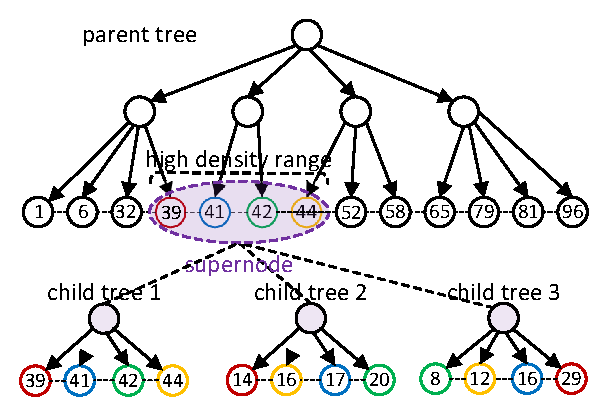
\includegraphics[width=2.8in]{fig/layerlsb.eps}}
    \caption{An illustrative example of LayerLSB structure. The circles with the same color indicate the same original data point. The number inside each circle is the $z$-value of that point in a particular LSB-tree.}
    \label{fig:layerlsb}
\end{figure}

We propose LayerLSB structure by exploring the density of $z$-values. Since the queries falling in high density range usually show low search quality, extra efforts are put into building indices for these queries. Fig. \ref{fig:layerlsb} shows an illustrative example of LayerLSB structure. The leaf nodes in high density ranges are rehashed in multiple independent child LSB-trees. These leaf nodes in parent tree are merged as a \emph{supernode}. The original $z$-value\footnote{The common representation of a $z$-value is a binary string. For ease of exposition, we use a positive integer to represent a binary string for demonstrating the tightness of leaf entries.} obtained in parent LSB-tree are retained in the first child tree. Two extra child trees with a new set of LSB parameters are further created. As a result, new $z$-values of these rehashed data points are obtained.

Even though only two levels are shown in Fig. \ref{fig:layerlsb}, it is possible to further rehash the level-1 child LSB leaf nodes and create level-2 child LSB-trees. This results a \emph{multi-layered} LSB-trees structure. This variation of $z$-values' order achieved by extra LSHs will increase the probability of returning real $k$NNs. Comparing to blindly createing more LSB-trees without discrimination, great effort can be saved by targeted rehashing. A small number of root level LayerLSB-trees is enough to obtain a high search quality. Next, we will describe how to build the LayerLSB structure.


\subsection{Building LayerLSB-Tree}

\Paragraph{Range Density Evaluation} To rebuild LSB-tree, evaluating the tightness of leaf neighbors is the first step. Recall that each leaf node is designated with a $z$-value. We use \emph{z-value range density} to quantify the tightness of leaf neighbors. It is straightforward to make a histogram to estimate the range densities where the length of each bin indicates the number of $z$-values in that range. Thus, the leaf nodes in dense ranges can be identified for further rehashing.

\Paragraph{Child LSB Parameters Determination} The identified high density leaf nodes are going to be inserted into multiple independent child LSB-trees. With respect to the parameters setting in child LSB, the dimensionality $m_{c}$ of $G(o)$ is set as $m_{c}=log_{1/p_2}{\frac{dn}{B}}$ (where $p_2$ is a constant probability under an approximation ratio and $B$ is the page size for external storage) \cite{lsb} and the partition width is consistent with its parent tree. Since the number of child tree points $n$ is much smaller than that in parent tree, $m_{c}$ is a small number, and the length of each $z$-value is greatly reduced. This results in a smaller index for child LSB-trees. In addition, we leave the number of child trees $l_{c}$ as a user-defined parameter as it balances the tradeoff between search quality and search cost.
%We will empirically show the effect of $l_{c}$ in Sec. \ref{sec:expr:param}.

\Paragraph{Child LSB-Tree Generation} With regard to every point in a high density range, a number $l_{c}$ of $z$-values are computed and inserted into these child LSB-trees respectively. The child tree generation process is executed recursively until no dense range exists. It is noticeable that too many levels will take up too much space and degrade query performance. Fortunately, it is common that only one child LSB level is enough to achieve high search quality.


\subsection{Query Processing}

%The query processing in LayerLSB is a simple extension of the that in original LSB. We first review the query processing in the original LSB. The LSB uses the \emph{length of the longest common prefix} (LLCP) of $z(q)$ and $z(o)$ denoted by $LLCP(z(q), z(o))$ to quantify the similarity of two $Z$-value $z(q)$ and $z(o)$. Recall that the $Z$-value $z(o)$ is a binary string. The larger of the $LLCP(z(q), z(o))$ is, the more likely that $o$ is similar to $q$. The nearest neighbor algorithm in original LSB performs a synchronous bi-directional expansion at the leaf levels of all trees and visits leaf entries in descending order of their LLCPs to $z(q)$.

\begin{algorithm}[t]
\SetKwData{Query}{$q$}\SetKwData{Heap}{$H$}\SetKwData{Entry}{$e$}\SetKwData{CandidateSet}{$S$}
\SetKwProg{Fn}{Function}{:}{end}
\SetKwFunction{FindEntryInTrees}{FindNodeInTrees}
\SetKwInOut{Input}{input}\SetKwInOut{Output}{output}

\Input{query \Query, LayerLSB trees $\{T^0_1,T^0_2,\ldots,T^0_l\}$}
\Output{$k$NN candidates set \CandidateSet}
\BlankLine
initialize a min-heap \Heap and a set \CandidateSet\;
\FindEntryInTrees(\Query, $\{T^0_1,T^0_2,\ldots,T^0_l\}$, \Heap)\;
\While{not terminated}{\
    \Entry $\leftarrow$ \Heap.pop()\;
    insert \Entry into \CandidateSet\;
    \tcc{from parent tree to child trees}
    \uIf{\Entry.next is a supernode}{\
        \FindEntryInTrees(\Query, \Entry.next.ctrees, \Heap)\;
    }
    \tcc{from child tree to parent tree}
    \uElseIf{\Entry.next is left/right-most leaf node}{\
        \If{\Entry.supernode is not null}{\
            push \Entry.supernode.next into \Heap\;
        }
    }
    \Else{
        push \Entry.next into \Heap\;
    }
}
return \CandidateSet;
\BlankLine
\BlankLine
\Fn{\FindEntryInTrees{\Query, $\{T_1,T_2,\ldots\}$, \Heap}}{\
    \ForEach{$T_i$ in $\{T_1,T_2,\ldots\}$}{\
        compute $z_i(\Query)$ in $T_i$\;
        \eIf{$z_i(\Query)$ belongs to a supernode}{\
            \FindEntryInTrees(\Query, supernode.ctrees, \Heap)\;
        }{
            locate $e\vdash_i$ and $e\dashv_i$ in $T_i$ based on $z_i(\Query)$\;
            push $e\vdash_i$ and $e\dashv_i$ into \Heap\;
        }

    }
}
\caption{The $k$NN algorithm in LayerLSB}
\label{alg:layerlsb_query}
\end{algorithm}

The query processing in LayerLSB is similar to that in original LSB. Both rely on bidirectional expansion. But there is a key difference between them, which is that in LayerLSB the expansion might move between parent tree and child trees. We describe the query algorithm of LayerLSB in Algorithm \ref{alg:layerlsb_query}.

We use a min-heap $H$ to maintain the leaf nodes in descending order of their LLCP with $q$ (Line 1). Denote the $l$ root-level (or level-0) LSB-trees as $T^0_1,T^0_2,\ldots,T^0_l$ respectively. We first search each root-level tree $T^0_i$ to locate the leaf node $e\vdash_i$ with the lowest $z$-value at least $z_i(q)$ (i.e., right-moving node) and the leaf node $e\dashv_{i}$ with the highest $z$-value at most $z_i(q)$ (i.e., left-moving node and preceding node of $e\vdash_i$) (Line 23,24). If $z_i(q)$ falls into a high density range, i.e., $z_i(q)$ belongs to a supernode that links to multiple child trees, we will recursively compute $q$'s $z$-values in child trees and locate the corresponding left-moving and right-moving nodes that will be pushed into $H$ (Line 21).

Next, we pop the first node $e$ from $H$ which has the largest LLCP with $q$ (Line 4). The moving direction information is embedded in node $e$ such that $e$.next will return $e$'s left-sibling node or right-sibling node. If $e$.next falls into a low density range, i.e., $e$.next belongs to a supernode and links to multiple child trees, we should move the cursor from parent tree to child trees. A recursive \texttt{FindNodeInTrees} process is invoked to search leaf nodes in child trees (Line 6). If $e$.next happens to be the left-most/right-most node of the tree, which means that all the leaf nodes preceding/following $z(q)$ have been visited in that tree, we should move the cursor from child tree to parent tree unless it is already root-leveled. The left/right sibling leaf node of the supernode where $e$ falls is pushed into heap $H$ (Line 10). Otherwise, $e$.next is a leaf node at the same level as $e$ such that $e$.next is simply pushed into $H$. This bidirectional expansion process continues until a certain termination condition is satisfied. All the popped nodes from $H$ are considered as $k$-NN candidates and returned for further distance measurement.

\begin{comment}
\begin{figure}[htb]
    \centerline{\includegraphics[width=3.4in]{fig/layerlsb_query.eps}}
    \caption{An illustrative example of query process in LayerLSB with a single parent tree and 3 child trees. The upper part shows the global LLCP order in both parent tree and child trees. We move left or right one position each step. The number above the moving direction means the moving step. }
    \label{fig:layerlsb_query}
    \vspace{-0.1in}
\end{figure}

Fig. \ref{fig:layerlsb_query} shows an illustrative example. Only the leaf levels of parent tree and child trees are drawn. The supernode at parent tree level links to the 3 child trees. The moving between parent tree and child trees should be noticeable. 1) When moving from parent tree to child trees, new $z$-values of $q$ are computed with child LSB parameters, and the LLCPs with left/right sibling node in child trees should be reevaluated. 2) When moving from child tree to parent tree, the parent-level node is visited only for the first time from child tree to parent tree, since multiple child trees linked from the parent tree.
\end{comment}

Note that, the query in LayerLSB structure will not impact LSB's theoretical quality guarantee. We just create more targeted child trees for part of the parent tree. As long as we sustain the termination condition $E_1$ and $E_2$, the collision probability will not be impacted.

%\Paragraph{Quality Guaranteed Approximate Query Processing}
%The original LSB endows with a very good property that performs approximate NN query with quality guarantee. This is achieved by carefully setting parameters and fulfilling termination condition $E_1$ and $E_2$ as discussed in Sec. \ref{sec:reclsb:review}. To guarantee search quality with the multi-level tree structure in LayerLSB, we accordingly set LSH parameters and sustain the termination condition $E_1$ and $E_2$. The parameters of level-0 LSB trees are set consistent with the original LSB, i.e., $l=\sqrt{dn/B}$ and $m=log_{1/p2}(dn/B)$. With regard to the higher level trees, $m$ is set the same as level-0 tree, and $l$ is a user-specified number. It is obvious that as long as the same termination condition $E_1$ and $E_2$ are fulfilled, the expected quality of LayerLSB is no lower than the original LSB no matter what $l$ is. To satisfy $E_1$, we ensure that the number of leaf entries accessed from all level-0 trees plus the number of unique leaf entries accessed from all child trees has reached $4Bl/d$. On the other hand, we can assure $E_2$ by ensuring that the nearest point found so far has distance to $q$ at most $2^{u-\lfloor v/m\rfloor+1}$.

\begin{comment}
\subsection{Index Maintenance}

LSB-tree is originally a disk-based index. The core is a B-tree structure. For supporting bidirectional expansion operation, the leaf node stores pointers to its left sibling and right sibling. The insertion and deletion are well supported in the conventional B-tree structure. LayerLSB index structure follows the design of LSB. Besides, 1) for supporting the moving operation between parent tree and child trees, the left/right neighbor node of a supernode stores pointers to the leftmost/rightmost nodes of child trees, and vice versa. In addition, 2) the leaf node (with $z(o)$) contained in a supernode stores pointers to its corresponding leaf nodes (with $z_j(o)$) in child trees, so the location of a query in multiple child trees can be achieved through much fewer I/O operations.
\end{comment}

